%%% lorem.tex --- 
%% 
%% Filename: lorem.tex
%% Description: 
%% Author: Ola Leifler
%% Maintainer: 
%% Created: Wed Nov 10 09:59:23 2010 (CET)
%% Version: $Id$
%% Version: 
%% Last-Updated: Wed Nov 10 09:59:47 2010 (CET)
%%           By: Ola Leifler
%%     Update #: 2
%% URL: 
%% Keywords: 
%% Compatibility: 
%% 
%%%%%%%%%%%%%%%%%%%%%%%%%%%%%%%%%%%%%%%%%%%%%%%%%%%%%%%%%%%%%%%%%%%%%%
%% 
%%% Commentary: 
%% 
%% 
%% 
%%%%%%%%%%%%%%%%%%%%%%%%%%%%%%%%%%%%%%%%%%%%%%%%%%%%%%%%%%%%%%%%%%%%%%
%% 
%%% Change log:
%% 
%% 
%% RCS $Log$
%%%%%%%%%%%%%%%%%%%%%%%%%%%%%%%%%%%%%%%%%%%%%%%%%%%%%%%%%%%%%%%%%%%%%%
%% 
%%% Code:

\chapter{Method} \label{cha:method}
Now that the theoretical groundwork has been laid out, we describe in \cref{sec:implementation} how the solution was implemented into Configura's graphics pipeline and then show how to evaluate it in \cref{sec:evaluation}.

\iffals
In more detail, the implementation description shows how the different algorithms are implemented in practice and how these fit into Configura's pipeline. Moreover, we also show how the appearance evaluator has been implemented and integrated into the system. In the evaluation part of the method, we describe how to measure the computation time, memory usage, polygon count and appearance preservation of a algorithm given a certain mesh and parameters.
\fi

\section{Implementation} \label{sec:implementation}
OVERVIEW

\subsection{Handling seams}
To be able to apply a texture to a mesh a mesh parameterization is needed that maps vertices to texture coordinates. If the mesh is not homeomorphic to a disk it is split into parts which will introduce seams. Vertices along these seams is duplicated which enable us to have multiple texture coordinates. However, this is a problem during simplification and will likely make the mesh tear in the seams. Welding duplicate vertices removes the seams and our tearing problem goes away. This, however, does not work good for textured meshes since we can no longer have discontinuities. Vertices that share the same attributes are safe to remove though.

\begin{figure}[h]
    \centering
    \includegraphics[width=.5\textwidth]{figures/mesh_tear.png}
    \caption{Mesh tear in seam}
    \label{fig:mesh_tear}
\end{figure}

The mesh representation by Hoppe \cite{hoppe1998efficient} allows vertices to have multiple attributes associated with it. As explained in \cref{sec:vertex_with_multi_attributes} the corners of a face defines the attribute value that should be used for that face.

\begin{figure}[h]
    \centering
    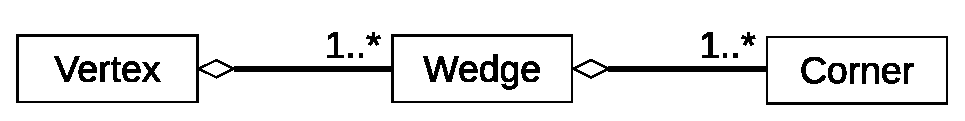
\includegraphics[width=.5\textwidth]{figures/vertex_wedge_corner.eps}
    \caption{Multi-attribute vertex}
    \label{fig:vertex_wedge_corner}
\end{figure}

\subsubsection{Finding duplicate vertices}
A fast method to find vertices that occupy the same space in 3D is to use a hash map. It is an associative container that is organized into buckets that contains the elements. Search, insert, and removal of elements have on average constant time complexity but in the worst case linear. If a key maps to the same bucket as another key it will be put in a collision chain in the same bucket. The time complexity will in that case be linear on the number of elements in that bucket.

To get fast search and insert a hash function with few collisions is important. The hash function that is used at Configura can be seen in \cref{lst:hash3D}. This hash of a 3-dimensional vector is a combination of the x, y, z coordinates. The hashes of x and y is also rotated i.e. bits are circular shifted, to get fewer collisions. 

\lstset{
  language=C++,
  classoffset=0,
  morekeywords={in,from,to},
  keywordstyle=\bfseries\color{blue},
  commentstyle=\itshape\color{darkgreen},
  classoffset=1,
  morekeywords={hash,floor,rotateRight,eq,abs,removeDuplicates},
  keywordstyle=\bfseries\color{darkblue},
  classoffset=2,
  emph={int,float,vec2,vec3,bool,double,vector,void},
  emphstyle={\bfseries\color{darkred}},
  classoffset=3,
  emph={V,U},
  emphstyle={\bfseries\color{black}},
  classoffset=0,
  captionpos=b}
\begin{minipage}{\linewidth}
\begin{lstlisting}[caption={Hashing 3D point}, label={lst:hash3D}]
  bool eq(float a, float b) {
    return abs(a - b) < precision;
  }
  
  int hash(float z) {
    if (eq(z, 0.0)) return 0;
    float r = floor(z/precision);
    int* p = (int*)&r;
    return rotateRight(p[0], 4);
  }
  
  int hash(vec3 p) {
    return (rotateRight(hash(p[0]), 8) +
            rotateRight(hash(p[1]), 4) +
            hash(p[2]));
  }
\end{lstlisting}
\end{minipage}

Extracting all \emph{unique} vertices in a mesh can be done with the aformentioned hash map. This is done by iterating through all the vertices and inserting them into the hash map. If the map already contains a vertex we have found a duplicate and it will not be inserted. After the iterations the map will only contain unique vertices and the next step is to update the triangles to map to the new vertices. This is an easy task since when the vertices are inserted into the hash map they will be associated with an index. Therefore, we only have to iterate through the triangle indices and update them with the new indices. (See \cref{lst:remove_duplicates}).

\begin{minipage}{\linewidth}
  \begin{lstlisting}[caption={Removing duplicates}, label={lst:remove_duplicates}]
    void removeDuplicates(vector<vec3>& vertices,
                          vector<int>& triangles) {
      unordered_map<vec3, int> indices;
      vector<vec3> newVertices;
      
      for (vec3 v : vertices) {
        if (!indices.count(v)) {
          indices.emplace(v, newVertices.size());
          newVertices.push_back(v);
        }
      }

      vertices = newVertices;

      // Remap triangles to the new vertices
      for (int i=0; i<triangles.size(); i++) {
        int index = triangles[i]
        vec3 z = vertices[index];
        int newIndex = indices[z];
        triangles[i] = newIndex;
      }
    }
\end{lstlisting}
\end{minipage}

\iffalse
% Too long!? Move to appendix?
\begin{minipage}{\linewidth}
  \begin{lstlisting}[caption={Removing duplicates}, label={lst:remove_duplicates}]
    void removeDuplicates(vector<vec3>& vertices,
                          vector<vec2>& texCoords,
                          vector<int>& triangles) {
      unordered_map<vec3, vector<int>> indices;
      unordered_map<int, int> old_to_new;
      
      vector<vec3> newVertices;
      vector<vec2> newTexCoords;
      
      for (int i=0; i<vertices.size(); i++) {
        vec3 v = vertices[i];
        vec2 t = texCoords[i];
        
        if (!indices.count(v)) {
          vector<int> vec{newVertices.size()};
          indices.emplace(v, vec);
          oldToNew.emplace(i, newVertices.size());
          
          newVertices.push_back(v);
          newTexCoords.push_back(t);
          
        } else {
          vector<int> vec = indices[i];
          
          if (uniqueTexCoord(i, vec)) {
            indices[v].push_back(newVertices.size());
            oldToNew.emplace(i, newVertices.size());
            
            newVertices.push_back(v);
            newTexCoords.push_back(t);
          }
        }
      }

      vertices = newVertices;
      texCoords = newTexCoords;

      // Remap triangles to the new vertices
      for (int i=0; i<triangles.size(); i++) {
        int index = triangles[i];
        triangles[i] = oldToNew[index];
      }
    }
\end{lstlisting}
\end{minipage}
\fi

\subsubsection{Vertices with multiple attributes}
To handle vertices with multiple unique attributes the \texttt{removeDuplicates} function require some modification. A simple solution is to associate each 3-dimensional vector with an array of indices. Thus, vertices can be associated with multiple texture coordinate indices. A vertex will only be removed if it is in the same place as another vertex with the same texture coordinates. However, if the texture coordinate is unique the vertex index will be added to the end of the list associated with the spatial coordinate.

This association can then be used to create vertices divided into one or more wedges. This kind of vertex will hereafter be called \emph{multi-vertex} to distinguish it from the real vertices. For each vertex, a wedge will be created containing the vertex index and then put in an array. A multi-vertex will contain indices to this array of wedges. 

\subsection{Solving linear equation systems}
A very common task during the simplification is to find the optimal position for a vertex after an edge collapse. As mentioned in \cref{sec:quadric-based_error_metric}, this is done by solving the linear equation system \(A v_{min} = b\) where \(v_{min}\) is the optimal position. In the original version of the QEM the optimal solution is obtained by finding \(A^{-1}\). If the matrix \(A\) is not invertable one of the vertices on the end points of the edge is chosen to be the new position.

In MixKit, the inverse of a matrix is found using Gaussian elimination with partial pivoting. The method is fast but it was noted that in many cases it fails to find the inverse of the matrix. This leads to many fallbacks to the endpoints which may give bad results for vertices with multiple attributes.

In order to have a higher rate of found solutions to the linear equation systems the linear algebra library \emph{Eigen} \footnote{\href{http://eigen.tuxfamily.org}{eigen.tuxfamily.org}} was used. This library contains numerical solvers, some more accurate and some with higher speed. First, the solvers finds a decomposition of $A$ and then the decomposition is used to find a solution. The choice of a solver is a tradeoff between speed and accuracy. A fast but also with decent accuracy is a solver using LU decomposition with partial pivoting and is a good candidate for the optimization problem. 

\subsection{Quadric-Based Error Metric} \label{sec:quadric-based_error_metric2}

As a rule, the original mesh will be given as an ordinary triangle mesh (a so called ``triangle soup''), which is not suitable for applying the QEM algorithm (since the local neighborhood information isn't available). Instead, we convert this triangle soup to a half-edge mesh. This allows easy manipulation of the local neighborhood of the mesh, which is precisely what is needed when doing an edge collapse or when calculating the error quadrics of a given vertex.

After doing this, the implementation basically follows the theoretical framework to the letter, where the least-cost edge is chosen to be contracted from the min-heap. Lastly, this edge is collapsed and then the remaining ``hole'' is simply (but with a few special cases...) linked back together so that the local neighborhood of the vertex still qualifies as a closed manifold.

\iffalse
\subsection{Integrating Solution into the Pipeline} \label{sec:integrating_solution_into_the_pipeline}

When the candidate algorithm has been chosen, it has to be integrated into CET Designer. Since we've chosen to evaluate the solution in C/C++ in our own renderer, the algorithm needs to be ported to the Configura CM language. It also needs to interact with the existing file format of the models, which means that either an existing Configura library will be needed or a custom one will need to be written for our purposes. After that, the integration is mostly painless, because the algorithm doesn't depend that much on any of the other parts in CET Designer. It should just be a case of: \emph{original mesh} $\rightarrow$ \emph{mesh simplifier} $\rightarrow$ \emph{simplified mesh}.
\fi

\section{Evaluation} \label{sec:evaluation}
OVERVIEW

\iffalse
In order to determine which of these algorithms provide the best performance for a target appearance threshold, an evaluation of the polygon count, computation time, memory usage and rendering time of the simplified mesh is done for each of the implemented solutions. In the results from this step, a series of tables are generated to compare the performance between the algorithms by using a common comparison framework. In this section, we describe this common comparison framework and then show how we can measure each of the parameters.

In essence, this is done by targeting a certain appearance threshold, tweaking the mesh simplification algorithm's parameters to achieve this threshold, and then measuring the given performance. This gives a universal measure of ``quality'' for all of the algorithms, which would otherwise have different error metrics used for applying the simplification. Since the performance measures are noisy, a total of \(n=20\) samples will be taken. According to \emph{David Lilja}~\cite[p.~50]{lilja2005measuring} the t-student distribution should be used when \(n < 30\), as shown in Section~\ref{sec:measuring_algorithmic_performance}.

The pack of test meshes that are going to be used in the comparison are a combination of textured models provided by Configura and others taken from the public domain. The exact selection of these is still to be decided, but should include both low- \& high-polygon meshes.
\fi

\iffalse
\subsection{Appearance Preservation} \label{sec:appearance_preservation}
In order to compare the appearance preservation of the mesh simplification algorithms, the image-metric explained in section~\ref{sec:metrics_for_appearance_preservation} is used. It is useful since it can compare the difference of any two meshes, therefore, it does not depend on the algorithm used.

For both the original mesh and a simplified mesh, 24 images with resolution $512 \times 512$ is rendered with a simple renderer based on \emph{OpenGL}. The camera is placed at the vertices of a rhombicuboctahedron and is faced towards the center where the mesh is placed. A light source is placed at the camera position. This will make sure that the surface facing the camera will be illuminated.

The two sets of 24 images each is used to compute the RMS of the simplified mesh with equation~\ref{eq:rms_image_sets}. This RMS value can then be used to compare how well the algorithms perform. 
\subsection{Polygon Count} \label{sec:polygon_count}
Concerning research question 3, the appearance preservation for a specific target polygon count needs to be measured. Therefore, the simplification algorithms is tasked to simplify until the target polygon count is reached. When it is reached, the image-metric is used to measure how well the appearance is preserved. Measurements will be performed for multiple target polygon counts. 

\subsection{Computation Time} \label{sec:computation_time}

An important property of a mesh simplification algorithm is the time it takes to simplify a full-resolution mesh to a lower-resolution mesh. While this doesn't impact the run-time of the mesh (that is accounted for by the rendering time, measured in Section~\ref{sec:rendering_time}), it is still important to reduce it as much as possible. This is especially true if the LoD is dynamically generated at run-time, but it is also important since many more meshes can be simplified per time unit (important if a simplifier is to be provided as a service, as \emph{Simplygon Linköping} does).

In order to compare the execution time of the different algorithms, they all target the same appearance thresholds as specified in Section~\ref{sec:appearance_preservation} by tweaking the parameters unique to each algorithm. We then measure the time it takes for the simplification algorithm to execute when using these parameters, in other words, simply by: \(time_\mathcal{A} = end_\mathcal{A} - start_\mathcal{A}\) for an algorithm \(\mathcal{A}\). Of course, this measurement is done several times to account for noise. After calculating the mean \(\bar{x}\) and the standard-deviation \(s\), one can find the confidence interval \([a, b]\) of the execution time by the equations shown in Section~\ref{sec:measuring_algorithmic_performance} with 19 degrees of freedom and \(\alpha = 5 \%\).

\subsection{Memory Usage} \label{sec:memory_usage}

Another important performance property of the algorithm is the accumulated memory used when simplifying the mesh. Depending on the size of the mesh in triangles, the algorithm could consume large amounts of memory (and might not even fit in the primary memory in some cases). It is therefore important to compare the simplification algorithms to determine those which are suited for optimizing large triangle meshes and those that aren't. Since this measure will always be deterministic (at least for the method we use to measure it), there is no need to apply any statistical measures. The \emph{Valgrind} suite was chosen since it has the \emph{Massif} heap profiler, which gives accurate memory usage. According to the \emph{Massif documentation}~\cite{valgrind2017manual} there is an expected slowdown of 20x, which isn't a problem since the computation time and rendering time are measured separately. Below are the commands to find the memory usage.

\begin{lstlisting}[language=bash]
  (*\textbf{valgrind}*) --tool=massif (*\textit{./simplify --algorithm=<algorithm> <input-mesh> <output-mesh>}*)
\end{lstlisting}

\subsection{Rendering Time} \label{sec:rendering_time}
One main purpose of simplifying a mesh is to reduce the rendering time. Therefore, the frame rate is measured when rendering the original mesh and the simplified meshes. The simplified meshes comes from the previous steps where different appearance-thresholds was targeted. Frame rate is measured by counting how many frames that have been rendered during a period of one second. As with computation time, this measurement may have noise and therefore multiple samples needs to be obtained. The mean and confidence interval is obtained in the same way.
\fi

%%%%%%%%%%%%%%%%%%%%%%%%%%%%%%%%%%%%%%%%%%%%%%%%%%%%%%%%%%%%%%%%%%%%%%
%%% method.tex ends here

%%% Local Variables: 
%%% mode: latex
%%% TeX-master: "thesis"
%%% End: 
